% The coupling agreed with Oliver on 20 Oct 2026: key points only (MEETING_2026-10-20.md).
% Build: pdflatex slides_coupling_1020.tex (twice). Rules: CLAUDE.md "Slides, notes and other documents".
\documentclass[aspectratio=169,11pt]{beamer}
\usetheme{Madrid}
\usecolortheme{seahorse}
\usepackage{booktabs}
\usepackage{amsmath,amssymb}
\usepackage{xcolor}
\usepackage{tikz}
\usetikzlibrary{arrows.meta,positioning}

\definecolor{c3}{RGB}{30,80,160}
\definecolor{warn}{RGB}{200,30,30}
\tikzset{box/.style={draw,rounded corners,align=center,font=\footnotesize,minimum height=1.0cm,text width=#1},
  box/.default=3.6cm, arr/.style={-{Latex[length=2mm]},thick}}
\setbeamercolor{frametitle}{bg=c3, fg=white}
\setbeamertemplate{navigation symbols}{}

\title{Coupling the Point Model to the Growth Field}
\subtitle{Key points of the meeting of 20 October 2026}
\author[Keisuke Nishioka]{Keisuke Nishioka}
\institute[IKM, LUH]{\small Institute of Continuum Mechanics (IKM), Leibniz Universit\"at Hannover}
\date{20 October 2026}

\begin{document}
\maketitle

% --------------------------------------------------------
\begin{frame}{What changes}
\begin{itemize}\setlength{\itemsep}{6pt}
  \item The point model of Klempt et al.\ 2026 is used \textbf{as published}: equations, parameters and its
        constraint $\sum_i\phi_i+\phi_0=1$ unchanged. It is called at every Gauss point with given inputs and
        returns its state.
  \item No longer: scaling the point model to the field amount ($\phi_0=1-\phi_{3D}$).
  \item Field to point model: nutrient $c^*$ and antibiotic $\alpha^*$ from 3D fields, interpolated in time.
  \item Point model to field: only the living biomass consumes nutrient and takes up antibiotic.
  \item Growth law Eq.\ 36 unchanged; Eq.\ 34 with its front term, so the nutrient reaches growth and stress.
  \item Into the thesis (Chapter 4), replacing the earlier coupling.
\end{itemize}
\end{frame}

% --------------------------------------------------------
\begin{frame}{The loop at one Gauss point}
\centering
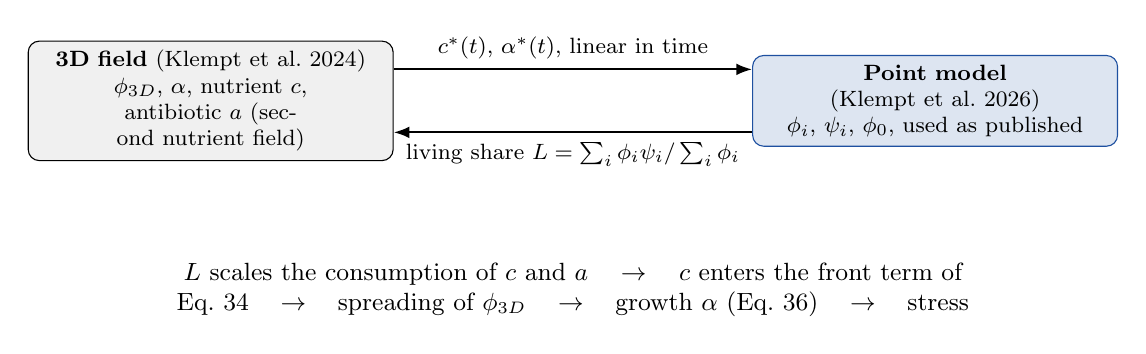
\begin{tikzpicture}
\node[box=4.4cm,fill=gray!12] (f) at (0,0) {\textbf{3D field} (Klempt et al.\ 2024)\\ $\phi_{3D}$, $\alpha$, nutrient $c$,\\
  antibiotic $a$ (second nutrient field)};
\node[box=4.4cm,fill=c3!15,draw=c3] (p) at (9.2,0) {\textbf{Point model} (Klempt et al.\ 2026)\\
  $\phi_i$, $\psi_i$, $\phi_0$, used as published};
\draw[arr] ([yshift=4mm]f.east) -- node[above,font=\footnotesize]{$c^*(t)$, $\alpha^*(t)$, linear in time}
  ([yshift=4mm]p.west);
\draw[arr] ([yshift=-4mm]p.west) -- node[below,font=\footnotesize]{living share $L=\sum_i\phi_i\psi_i/\sum_i\phi_i$}
  ([yshift=-4mm]f.east);
\node[align=center,font=\small,text width=13cm] at (4.6,-2.4) {
  $L$ scales the consumption of $c$ and $a$ $\;\to\;$ $c$ enters the front term of Eq.\ 34 $\;\to\;$
  spreading of $\phi_{3D}$ $\;\to\;$ growth $\alpha$ (Eq.\ 36) $\;\to\;$ stress};
\end{tikzpicture}
\end{frame}

% --------------------------------------------------------
\begin{frame}{Equations}
\small
\begin{align*}
&\text{inputs, } t_n\le t\le t_{n+1}: &
c^*(t)&=c^*_0\Bigl[\tfrac{t_{n+1}-t}{\Delta t}c_n+\tfrac{t-t_n}{\Delta t}c_{n+1}\Bigr],\quad
\alpha^*(t)=\alpha^*_0\,a(t)\ \text{likewise}\\[2pt]
&\text{nutrient (Eq.\ 35):} & 0&=d\,\nabla^2c-g\,\phi_{3D}\,L\,c\\
&\text{antibiotic:} & 0&=d_a\nabla^2a-g_a\,\phi_{3D}\,L\,a\\
&\text{spreading (Eq.\ 34):} & \dot\phi&=\beta\nabla^2\phi+k_\alpha\alpha
  -\|\nabla\phi\|\,\tfrac{r\,c}{k+c}\,\mathbf n_{\nabla\phi}\cdot\mathbf n_{\nabla c}\\
&\text{growth (Eq.\ 36):} & \dot\alpha&=k_\alpha\,\phi
\end{align*}
\begin{itemize}\setlength{\itemsep}{2pt}
  \item $L=1$ gives back Eq.\ 35; a dead biofilm ($L=0$) consumes nothing. $\phi_0$ has no living fraction.
  \item Eq.\ 35 is printed as $g\phi$; the implementation uses $g\phi c$ (misprint, confirmed).
  \item The antibiotic acts on the stress only indirectly: $\psi_i\downarrow\ \to L\downarrow\ \to c\uparrow\ \to$
        front term.
\end{itemize}
\end{frame}

% --------------------------------------------------------
\begin{frame}{Time: one clock for both models}
\begin{itemize}\setlength{\itemsep}{6pt}
  \item Klempt et al.\ 2024 normalise time with a reference time chosen for the problem. I choose
        $T^*=1$ as the duration of the point model's data.
  \item The point model then advances $s\,\Delta T^*$ per increment, with $s$ the length of that window in its
        own units: \textbf{$s$ follows, it is not fitted.}
  \item Synthetic data of Fritsch et al.\ 2025, case I: 1000 steps of $10^{-4}$, so $s=0.1$.
  \item Checked with synthetic data (four species): with its own constraint and $s$ from the window, the coupled
        point model reproduces the point model alone to $7\times10^{-7}$. Scaled to the field amount instead,
        the error is $0.019$, and a fitted $s$ comes out a third too low.
\end{itemize}
\end{frame}

% --------------------------------------------------------
\begin{frame}{Examples and checks}
\begin{columns}[T]
\begin{column}{0.48\textwidth}
\textbf{Examples} (synthetic, Fritsch et al.\ 2025 case I, two species, $b=(1,2)$)
\begin{itemize}\setlength{\itemsep}{2pt}\small
  \item A in the centre seed, B in the four vertical edges
  \item A and B mixed in the seed from the start
  \item nutrient from one wall, antibiotic from the opposite wall from $T^*=0.5$
  \item each with and without antibiotic
\end{itemize}
\end{column}
\begin{column}{0.5\textwidth}
\textbf{Checks}
\begin{itemize}\setlength{\itemsep}{2pt}\small
  \item uniform $c$ and $a$: the coupled point model equals the point model alone
  \item ANSYS against Python step by step (same inputs)
  \item $\phi$ stays in $[0,1]$ with the front term
  \item sensitivity: $\phi_{\min}$, coupling step, mesh
\end{itemize}
\textcolor{warn}{\small Python runs in progress; ANSYS on 21 October.}
\end{column}
\end{columns}
\end{frame}

% --------------------------------------------------------
\begin{frame}{Assumptions and open points}
\begin{itemize}\setlength{\itemsep}{5pt}
  \item \textcolor{warn}{Assumptions} (not in the papers): linear interpolation of $c^*$, $\alpha^*$ in time;
        $L$ from the previous increment; start values of newly reached points (mean state of the points the
        biofilm grows from); threshold $\phi_{\min}=0.01$.
  \item The point model has no transport between points: species A and B meet only through the start values
        of new points.
  \item The front term as printed moves the biofilm towards the nutrient; its large cell P\'eclet number needs
        upwinding (overshoot check).
  \item The calibrated five-species model has $b=0$ (no antibiotic in the data): the antibiotic is shown with
        synthetic data only.
\end{itemize}
\end{frame}

% --------------------------------------------------------
\appendix
\begin{frame}{Appendix: notation}
\small
\begin{tabular}{@{}ll@{}}
\toprule
$\phi_{3D}$, $\alpha$ & biofilm phase field and growth ($\mathbf F_g=\alpha\mathbf I$, $\alpha(0)=1$), Klempt et al.\ 2024\\
$c$, $a$ & nutrient and antibiotic fields (the element's first and second nutrient)\\
$d$, $g$, $d_a$, $g_a$ & diffusion and consumption of nutrient and antibiotic\\
$\beta$, $k_\alpha$, $r$, $k$ & diffusion of $\phi$, growth rate, front growth and Monod constant (Eq.\ 34, 36)\\
$\phi_i$, $\psi_i$, $\phi_0$ & volume fraction and living fraction of species $i$, auxiliary void (Klempt et al.\ 2026)\\
$c^*$, $\alpha^*$, $b_i$ & nutrient and antibiotic of the point model, antibiotic sensitivity\\
$L$ & living share of the point model's biomass, $\sum_i\phi_i\psi_i/\sum_i\phi_i$\\
$T^*$, $s$ & normalised time; point-model time per unit $T^*$\\
\bottomrule
\end{tabular}
\end{frame}

\end{document}
